\chapter*{Introduction}
\addcontentsline{toc}{chapter}{Introduction}
\chaptermark{Introduction}


\paragraph{Contextualisation\\}
Modèles cinétiques, dynamique des populations

Le développement de modèles mathématiques en sciences naturelles bénéficie toujours d'avancées mathématiques qui permettent de vérifier la caractère bien posé des équations, ou le bon comportement des solutions. Une classe de modèles très prisés depuis quelques dizaines d'années sont les modèles multi-échelles, dont l'étude principale se penche sur les modèles double-échelle. Dans ces modèles, on distingue deux dynamiques: une d'échelle caractéristiques $\eps$ et l'autre d'échelle $1$. Ce sont ces systèmes qui nous intéressent, et mathématiquement, ce manuscrit se concentre sur les problèmes qui prennent la forme 
\begin{equation} \label{sec:intro:eq:u}
  \pa_t u^\eps = -\frac{1}{\eps}A u^\eps + f( u^\eps ),
  \qquad u^\eps(0) = u_0 .
\end{equation}
On considère ce problème dans un Banach $(E, |\cdot|)$, avec $A : E \rightarrow E$ un opérateur linéaire et $f : E \rightarrow E$ un champ de vecteurs régulier. 

Ces modèles apparaissent en physique cinétique dans des espaces fonctionnels, avec $A$ qui est soit un opérateur de relaxation, soit un opérateur qui induit des oscillations~\cite{crouseilles.2017.nonlinear}. 

\bigskip
En général, on suppose $\eps \ll 1$, et donc la première dynamique est rapide par rapport à la seconde. À cet égard, des méthodes d'\textit{analyse asymptotique} ont été développées, c'est-à-dire des méthodes qui permettent de caractériser le système dans cette limite $\eps$ \enquote{petit}, en général en découplant ces deux dynamiques. Trois exemples particulièrement célèbres sont les méthodes d'homogénéisation, de moyennisation et de formes normales. 


\paragraph{Annonce de l'équation}
\begin{subequations} \label{sec:intro:eq:xz}
  \begin{empheq}[left=\left\lbrace, right=\right.]{align} &
    \pa_t x^\eps = a(x^\eps, z^\eps) , & &
    x^\eps(0) = x_0 , \vphantom{\frac11}\qquad\qquad
    \\ & 
    \pa_t z^\eps = -\frac{1}{\eps}\Lambda z^\eps + b(x^\eps, z^\eps) , & &
    z^\eps(0) = z_0 .
  \end{empheq}
\end{subequations}


Passage en notation $u^\eps$, 
\begin{equation} 
  \pa_t u^\eps = -\frac{1}{\eps} A u^\eps + f(u^\eps) .
\end{equation}

Présentation de ce qu'on entend par régime raide ou non-raide


\paragraph{Comportement de la solution\\}
En un temps assez court (de l'ordre de \eps), on rejoint un système de la 
forme 
\begin{subequations}
  \begin{empheq}[left=\left\lbrace, right=\right.]{align} &
    \pa_t x^\eps = a(x^\eps, \eps h^\eps(x^\eps)) 
    \\ &
    z^\eps = \eps h^\eps (x^\eps)
  \end{empheq}
\end{subequations}

Théorème de variété centrale

Figure de simulation de modèle jouet

\section*{Comportement théorique de la solution}
\addcontentsline{toc}{section}{Comportement théorique de la solution}

Dans cette section on décrit et illustre le comportement de la solution $(x^\eps, z^\eps)$. En particulier, on énonce le théorème de variété centrale, qui décrit le comportement de la solution en temps long, et on présente rapidement une méthode pour calculer cette variété centrale. On introduit ensuite quelques hypothèses qui permettront d'effectuer des approximations numériques dans la prochaine section. 


\subsection*{Observations de propriétés}
\addcontentsline{toc}{subsection}{Observations de propriétés}


Considérons le problème
\begin{equation} \label{sec:intro:pb:z_sin}
    \pa_t z(t) = -\frac{1}{\eps}z(t) + \sin(t), 
    \qquad
    z(0) = 1, 
\end{equation}
qui peut être transformé en un problème de la forme~\eqref{sec:intro:eq:xz} en posant $x(t) = t$, soit $\pa_t x = 1,\ x(0) = 0$. Ce problème peut être obtenu à partir de 
\begin{equation*}
    \pa_t y(t) = -\frac{1}{\eps} \big( y(t) - \cos(t) \big), 
    \qquad
    y(0) = 0, 
\end{equation*}
en posant $z(t) = y(t) - \cos(t)$. C'est un problème de référence pour l'introduction aux systèmes raides: c'est le premier exemple considéré dans~REF. La solution exacte se calcule sans difficulté en intégrant $\pa_t \big[ e^{t/\eps} z(t) \big]$, ce qui donne 
\begin{equation} \label{sec:intro:sol:z_sin}
    z(t) = e^{-t/\eps} \left( 1 + \frac{\eps^2}{1+\eps^2} \right)
        + \frac{\eps}{1 + \eps^2} \big( \sin(t) - \eps \cos(t) \big) .
\end{equation}

On observe que la solution comporte deux parties de nature différente, la phase transitoire (en $e^{-t/\eps}$) et la variété centrale (en $t$) de taille $\eps$. Ceci se voit sur la figure ci-dessous où on a tracé la solution et la variété centrale associée pour trois valeurs de~$\eps$. 

\begin{figure}[!h]
    \centering
    \includegraphics[width=.9\textwidth]{./Presentation/z_sin.pdf}
    \caption{Comportement de la solution~\eqref{sec:intro:sol:z_sin} pour différentes valeurs de~$\eps$, avec chaque variété centrale associée en pointillés.}
\end{figure}

\todo[inline]{Autre cas test où la dynamique sur $x$ change aussi}

\todo[inline]{Théorème de variété centrale}
En fait, dans le cas d'un système de la forme~\eqref{sec:intro:eq:xz}, la dynamique en temps long est déterminé entièrement par la variable $x$. Il y a une réduction de dimension, qui est traduite dans le théorème de variété centrale. 
\begin{FRtheorem*}[Variété centrale, REF]
    Si les fonctions $a,b$ sont de classe $C^1$, alors il existe un morphisme $x \mapsto z = \eps h^\eps(x)$, et un taux $\mu > 0$ tels que 
    \begin{equation*}
        \left| z(t) - \eps h^\eps\big( x(t) \big) \right|
        \leq e^{-\mu t/\eps} .
    \end{equation*}
    En outre, il existe une condition initiale \enquote{de l'ombre} $x_0^\eps$ telle que 
    \begin{equation*}
        \big| x(t) - \varphi_t^\eps \big( x_0^\eps \big) \big| 
        \lesssim \eps e^{-\mu t/\eps} , 
    \end{equation*}
    où $\varphi^\eps_t$ est le $t$-flot associé au champs de vecteur $x \mapsto a\big(x, \eps h^\eps(x) \big)$. On appelle l'ensemble des $\big( x, \eps h^\eps(x) \big)$ la variété centrale, qui attire la solution. 
\end{FRtheorem*}

Par exemple dans le cas~\eqref{sec:intro:pb:z_sin}, le morphisme de variété centrale $\eps h^\eps$ est donné par 
\begin{equation*}
    h^\eps(x) 
    = \frac{1}{1 + \eps^2} \big( \sin(x) - \eps \cos(t) \big) .
\end{equation*}
Il est impossible d'espérer calculer ce morphisme explicitement en général. On peut néanmoins appliquer une méthode de point fixe en remarquant qu'en temps long, et $z \approx \eps h^\eps(x)$ et d'où 
\begin{equation*}
    \pa_t z \approx \eps \pa_x h^\eps(x) \cdot \pa_t x
    \approx \eps \pa_x h^\eps(x) \cdot a(x, \eps h^\eps(x)) . 
\end{equation*} Ainsi on peut poser $h\rk 0 = 0$ et itérer de manière explicite
\begin{equation*}
    \eps \pa_x h\rk n(x) \cdot a(x, \eps h\rk n (x)) 
    = - h\rk{n+1}(x) + b(x, \eps h\rk n (x)) .
\end{equation*}
On remarque deux caractéristiques importantes de cette méthode: Elle nécessite de calculer une dérivée, ce qui demande du calcul symbolique potentiellement coûteux, et la convergence de la méthode n'est pas assurée. En effet, chaque itération vient demander un ordre de dérivation supplémentaire dans $a$ et $b$, ce qui peut croître comme $n!$ par exemple avec $a = 1$ et $b(x,z) = 1/(1+x)$. Même dans l'exemple jouet~\eqref{sec:intro:pb:z_sin}, cette méthode génère
\begin{equation*}
    h\rk{n}(x) = R_n(\eps) \sin(x) + \eps R_{n-1}(\eps) \cos(x) 
\end{equation*}
avec $R_n(\eps) = \sum_{k = 0}^{\left\lfloor n/2 \right\rfloor} \eps^{2k}$ et par convention $R_{-1} = 0$. En d'autres termes, on construit le développement en série entière en $\eps$ de la partie lente dans~\eqref{sec:intro:sol:z_sin}, i.e. $h\rk 1(x) = \sin(x)$, $h\rk 2 (x) = \sin(x) + \eps \cos(x)$ etc. Ainsi, le développement n'est convergent que pour $\eps < 1$, alors que le résultat de variété centrale est valide pour tout $\eps > 0$. 
%
Cette limitation apparaîtra couramment au cours de ce manuscrit sous le format plus contraignant
\begin{equation*}
    \eps \leq \frac{\eps_0}{n+1} ,
\end{equation*}
qu'on peut remarquer par exemple avec $b(x,z) = (1+x)^{-1}$ dont la taille des dérivées évolue de manière factorielle avec l'ordre de dérivation. 




\subsection*{Définitions et hypothèses}
\addcontentsline{toc}{subsection}{Définitions et hypothèses}


\todo[inline]{Problème uniformément bien posé}

\todo[inline]{Ouvert borné $\mathcal{K}$}

\todo[inline]{Régularité + \enquote{chaussette} autour de la solution}

\section*{Paradigme numérique}
\addcontentsline{toc}{section}{Paradigme numérique}

En général, on suppose $\eps \ll 1$, et donc le système~\eqref{sec:intro:eq:u} comporte une dynamique \textit{rapide} par rapport au temps d'étude. À cet égard, des méthodes d'\textit{analyse asymptotique} ont été développées, c'est-à-dire des méthodes qui permettent de caractériser le système dans cette limite $\eps$ \enquote{petit}, en général en découplant ces deux dynamiques. Pour les problèmes hautement oscillants, trois exemples particulièrement célèbres sont les méthodes d'homogénéisation~\cite{goudon.2003.homogenization}, de moyennisation~\cite{perko.1969.higher,sanders.2007.averaging,lochak.1988.multiphase} et de formes normales~\cite{murdock.2006.normal,bambusi.2003.birkhoff}. Pour les problèmes à relaxation rapide, la littérature est moins fournie. Qu'il s'agisse de calculer la variété centrale comme précédemment ou d'un développement de Chapman-Enskog~\cite{santos.1986.divergence,degond.2004.macroscopic,chartier.2015.uniformly}, la phase transitoire n'est pas calculée. 

Plus récemment dans \cite{castella.2016.formal}, les auteurs capturent
aussi la phase transitoire, mais la méthode n'est valide que dans la
limite $\eps \rightarrow 0$. Dans cette section, on étudie l'application
de méthodes numériques \enquote{standards} de l'état de l'art, et on
observe le comportement de l'erreur numérique non seulement en fonction
du pas de temps $\Dt$, mais aussi en fonction du paramètre $\eps$. 

On commence par décrire ce qu'on entend par \enquote{méthode numérique}
et le contexte dans lequel on va les étudier. Ensuite, on présente trois
méthodes d'ordre 2 de l'état de l'art~: le splitting de Strang, un
schéma IMEX-BDF et une méthode de Runge-Kutta exponentielle. 



\subsection*{Mise en place de la résolution}
\addcontentsline{toc}{subsection}{Mise en place de la résolution}

Pour étudier le comportement des schémas numériques sur les problèmes de la forme~\eqref{sec:intro:eq:u}, on considère l'exemple jouet suivant
\begin{subequations} \label{sec:intro:eq:jouet_v}
    \begin{empheq}[left=\left\lbrace, right=\right.]{align} &
        \pa_t v_1 = v_2 , & &
        v_1(0) = 1 , \vphantom{\frac11}\qquad\qquad
        \\ & 
        \pa_t v_2 = -\frac{1}{\eps}\big( v_1 + v_2 \big) , & &
        v_2(0) = 0 .
    \end{empheq}
\end{subequations}
Cet exemple ressemble à certains problèmes hyperboliques avec relaxation, et sa linéarité le rend simple à étudier. Il prend facilement la forme~\eqref{sec:intro:eq:xz} en posant par exemple $x = v_1$ et $z = v_1 + v_2 $, ce qui donne 
\begin{subequations} \label{sec:intro:eq:jouet_xz}
    \begin{empheq}[left=\left\lbrace, right=\right.]{align} &
        \pa_t x = -x + z , & &
        x(0) = 1 , \vphantom{\frac11}\qquad\qquad
        \\ & 
        \pa_t z = -\frac{1}{\eps}z - x + z , & &
        z(0) = 1 .
    \end{empheq}
\end{subequations}
Ce problème est linéaire et se diagonalise sans difficulté pour $\eps < 1/4$, ce qui génère
\begin{equation*}
    \newcommand{\sqEps}{\sqrt{1 - 4\eps}}
    \tilde{u} = \underbrace{\begin{pmatrix}
        -1 & 1 - r_\eps \\
        \eps & 1 - \eps - \eps r_\eps 
    \end{pmatrix}}_{\displaystyle P} \begin{pmatrix} x \\ z \end{pmatrix},
    \qquad\text{tel que}\qquad
    \pa_t \tilde{u} = \begin{pmatrix}
        -r_\eps & 0 \\ 0 & -\frac{1}{\eps} + r_\eps
    \end{pmatrix} \tilde{u}
\end{equation*}
avec $r_\eps = \frac{1}{2\eps} \big( 1 - \sqrt{1 - 4\eps} \big)$. On obtient ainsi une expression explicite pour $u = \among{x}{z}$ de la forme 
\begin{equation*}
    u(t) = P^{-1} \begin{pmatrix}
        e^{-t r_\eps} & 0 \\ 0 & e^{-t/\eps} e^{t r_\eps}
    \end{pmatrix} P u(0) 
\end{equation*}
où $P^{-1} = \frac{1}{\sqrt{1 - 4\eps}} \begin{pmatrix}
    -1 + \eps + \eps r_\eps  &  1 - r_\eps \\
                \eps         &      1
\end{pmatrix}$.
\begin{FRremark*}
    On voit bien dans la définition de $r_\eps$ que le problème change de nature entre $\eps \leq 1/4$ et $\eps > 1/4$. En effet, dans le premier cas le système est purement dissipatif, alors que dans le second, des oscillations apparaissent. Cette singularité apparaît également dans la matrice de changement de variable, dont le déterminant vaut $-\sqrt{1 - 4\eps}$.
\end{FRremark*}


En pratique, on ne sait pas résoudre tous les systèmes de la forme~\eqref{sec:intro:eq:u} de manière exacte. On va donc appliquer des méthodes d'\textit{approximation numérique} pour calculer une solution approchée. Plus spécifiquement, on va implémenter certains \textit{schémas numériques} et observer la qualité d'approximation sur l'exemple~\eqref{sec:intro:eq:jouet_xz}. Définissons ce qu'on entend par \enquote{schéma numérique}. 

On démarre par considérer une discrétisation de l'intervalle temporel $[0,T]$, c'est-à-dire qu'au lieu de considérer cet objet comme continu, on le considère comme une suite de $N+1$ points $(t_n)_{0 \leq n \leq N}$ avec $N \geq 1$. On choisit de se restreindre à une discrétisation \textit{uniforme}, c'est-à-dire que l'intervalle de temps $[0,T]$ est divisé en $N$ intervalles de taille égale notée $\Dt$. 
\begin{center}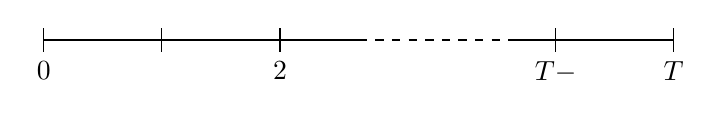
\begin{tikzpicture}
    \draw (0,0) -- (4,0);
    \foreach \x/\y in {0/$0$,1/$\Dt$,2/$2\Dt$} {
        \draw (\x*1.5,0.15cm) -- (\x*1.5,-0.15cm) node[below] {\y};
    }
    \draw[dashed] (4,0) -- (6,0);
    \draw (6,0) -- (8,0);
    \foreach \x/\y in {0/$T$,1/$T-\Dt$} {
        \draw (8-\x*1.5,0.15cm) -- (8-\x*1.5,-0.15cm) node[below] {\y};
    }
\end{tikzpicture}\end{center}
\vspace*{-12pt}
%
\noindent%
De manière équivalente, les points de séparation $(t_n)_{0 \leq n \leq N}$ sont donnés par 
\begin{equation*}
    t_{n+1} = t_n + \Dt
    \qquad\text{avec}\qquad
    t_0 = 0 \quad\text{et}\quad \Dt = \frac{T}{N} ,
\end{equation*}
ou encore $t_n = \frac{n}{N}T$. À cette discrétisation, on peut associer une \textit{approximation} $(u_n)_{0 \leq n \leq N}$ telle que $u_n \approx u(t_n)$. On peut voir un exemple d'une telle approximation en Figure~\ref{sec:intro:fig:approx_sin}, où les points carrés sont une approximation\footnote{Cette approximation est obtenue par itération en posant $\displaystyle z_{n+1} = z_n - \frac{\Dt}{\eps}z_{n+1} + \Dt \sin(t_n)$ avec $z_0 = z(0) = 1$, ce qui correspond à une méthode appelée IMEX-BDF1.} des points ronds. 

\begin{figure}[!ht]
    \centering
    \includegraphics[width=.9\textwidth]{./Presentation/approx_sin.pdf}
    \caption{Tracé de la solution exacte (en bleu, marqueurs ronds) au problème~\eqref{sec:intro:pb:z_sin} avec $\eps = 1$ et d'une approximation (orange, marqueurs carrés) sur une discrétisation uniforme de $[0,\pi]$ à 11 points.}
    \label{sec:intro:fig:approx_sin}
\end{figure}


\begin{FRdefinition*}
    On définit l'erreur d'une approximation comme l'erreur maximale sur les points d'interpolation, i.e. étant donnée une discrétisation à $N+1$ points $(t_n)_{0 \leq n \leq N}$ et une approximation $(u_n)$ d'une fonction $t \mapsto u(t)$, l'erreur est définie par la formule 
    \begin{equation} \label{sec:intro:def:err}
        \err = \max_{0 \leq n \leq N}\big| u_n - u(t_n) \big| .
    \end{equation}
    Si en outre la solution et l'approximation dépendent du paramètre~$\eps \in (0,\eps_0]$, on écrit $\err(\eps)$ l'erreur d'approximation, et on définit l'erreur uniforme $\overline{\err}$ par 
    \begin{equation}
        \overline{\err} = \sup_{\eps \in (0,\eps_0]} \err(\eps) .
    \end{equation}
    Ces deux erreurs peuvent avoir des comportements différents.
\end{FRdefinition*}
Parfois, l'erreur est définie comme l'erreur au temps final, ce qui peut paraître moins contraignant mais a peu d'influence en pratique car les estimations d'erreur sont croissantes avec l'indice~$n$. Ainsi ces deux définitions coïncident pour les résultats théoriques.

\begin{FRremark*}
    À partir d'une approximation $(u_n)$, on peut obtenir une approximation sur une discrétisation plus fine par interpolation (typiquement avec des splines cubiques ou de manière linéaire comme en Figure~\ref{sec:intro:fig:approx_sin}). Il semble alors naturel de se demander s'il est possible de réduire le coût de calcul en calculant une approximation sur une discrétisation grossière pour l'interpoler ensuite vers une discrétisation plus fine. Néanmoins, si l'erreur telle que définie en~\eqref{sec:intro:def:err} est mauvaise, on ne peut pas espérer l'améliorer par interpolation. C'est pourquoi ce manuscrit se concentre sur cette approche \enquote{simple} de l'erreur.
\end{FRremark*}

Lorsqu'il s'agit de trouver une approximation à une solution d'équation différentielle, il semble naturel de procéder de manière itérative: les seules données accessibles sont la condition initiale $u(0)$ et le champ de vecteurs suivi par la solution, donc il faut trouver un moyen de combiner ces deux informations pour obtenir une approximation $u_1 \approx u(\Dt)$. Une fois cette information obtenue, on peut l'utiliser avec les autres pour calculer $u_2 \approx u(2\Dt)$, etc. Dans les faits, on se limite à un nombre fixe $s \geq 1$ de points pour extrapoler le suivant. On parle alors de méthode multipoints. Les méthodes à un point sont appelées méthodes de Runge-Kutta.

La méthode utilisée pour calculer un terme à partir des précédents est appelé un schéma numérique~$\Phi^\eps_{\Dt}$, et elle peut s'écrire 
\begin{equation*}
    u_{n+s} = u_{n+s-1} + \Dt\, \Phi^{\eps}_{\Dt} (u_{n+s-1}, \ldots, u_n) .
\end{equation*}
Cette notation peut être pratique pour étudier le schéma, mais il faut garder à l'esprit qu'elle peut camoufler de nombreuses difficultés. Par exemple, le schéma d'Euler implicite s'écrit 
\begin{equation*}
    u_{n+1} = u_n + \Dt \left( 
        - \frac{1}{\eps}A u_{n+1} + f(u_{n+1}) 
    \right) .
\end{equation*}
Pour trouver $\Phi^\eps_{\Dt}$, il faut inverser cette relation; on parle de schéma \textit{implicite}, par opposition aux schémas \textit{explicites}. Cette inversion peut s'avérer particulièrement coûteuse si $f$ présente des non-linéarités et si le système est grand. Ainsi par la suite on se limite à des schémas \textit{explicites} en $f$, et on fait l'hypothèse suivante~:
\begin{FRassumption*}
    On sait calculer $t \mapsto e^{-tA}$ et $t \mapsto (\id + t A)^{-1}$ de manière exacte. 
\end{FRassumption*}
\noindent%
Calculer le semi-groupe $t \mapsto e^{-tA}$ peut sembler contraignant, mais rappelons nous qu'on se restreint ici au cas où $A$ est une matrice diagonale. 


\begin{FRdefinition*}
    On dit qu'un schéma numérique~$\Phi_{\Dt}$ est d'ordre $q$ s'il existe une constante $C > 0$ et un pas de temps maximal $\Dt_0 > 0$ tel que pour toute subdivision de pas de temps $\Dt \leq \Dt_0$, l'erreur de schéma est bornée par $C\Dt^q$. 
\end{FRdefinition*}
%
\noindent%
Dans le contexte d'un schéma qui dépend du paramètre~$\eps$, la constante d'erreur $C$ et le pas de temps maximal $\Dt_0$ dépendent généralement de $\eps$, ainsi il faut distinguer l'ordre du schéma (calculé pour $\Dt \ll \eps$) de l'ordre de \enquote{convergence uniforme} du schéma, qui fait disparaître la dépendance en~$\eps$. Cette distinction sera clarifiée par les exemples à venir.



\subsection*{Méthodes numériques}
\addcontentsline{toc}{subsection}{Méthodes numériques}

On présente les résultats associés à trois méthodes d'ordre 2, qui traitent la partie raide différemment de la partie non-raide. Les méthodes sont bien définies  dans la limite $\eps \rightarrow 0$, et on s'intéresse au comportement de l’erreur en fonction de $\Dt$ \textit{et} de $\eps$.

On ne considèrera pas de méthodes complètement implicites parce qu'elles sont très coûteuses notamment dans un contexte d'EDP. Néanmoins la convergence de ces méthodes est souvent excellente et des implémentations très efficaces existent. La référence sur le sujet est~\cite{hairer.1996.solving}, et toutes les bonnes boîtes à outils de résolution d'EDO contiennent la méthode RadauII.\footnote{Attention cependant, la plupart de ces boîtes à outils masquent la difficulté associée aux méthodes implicites, à savoir la résolution d'un système et l'erreur associée. En outre, il est parfois difficile de désactiver le pas de temps adaptatif, ce qui est problématique pour une étude de convergence.} On ne considère pas non plus de méthodes purement explicites demandant $\Dt < \eps$, ce qui est beaucoup trop coûteux en pratique. 

Il est important de noter que cette introduction ne présente pas une étude des schémas présentés. Il s'agit d'une compilation non-exhaustive de résultats et d'observations sur les propriétés de ces méthodes appliquées à~\eqref{sec:intro:eq:u} afin de contextualiser les contributions du manuscrit par la suite. Néanmoins, les schémas sont présentés plus en détails dans l'Annexe~\ref{chap:schemas}.



\paragraph{Splitting de Strang\\}

Une approche courante consiste à séparer le problème~\eqref{sec:intro:eq:u} en deux parties, l'une raide et l'autre non-raide. La manière naturelle de procéder fournit
%
\begin{empheq}[left=\left\lbrace, right=\right.]{align*} &
    \pa_t u^{(1)} = -\frac{1}{\eps}A u^{(1)} ,
    \\ &
    \pa_t u^{(2)} = f(u^{(2)}) . \vphantom{\frac11}
\end{empheq}
%
On note $\varphi_t$, $\varphi^{(1)}_t$ et $\varphi^{(2)}_t$ les $t$-flots associés aux problèmes en $u$, $u^{(1)}$ et $u^{(2)}$ espectivement. On remarque qu'il est simple de calculer $\varphi^{(1)}$ de manière exacte, et simple de calculer $\varphi^{(2)}$ de manière numérique. Cependant, ces deux dynamiques sont mélangées dans $\varphi$, ce qui rend le flot du problème d'origine difficile à calculer. Ainsi, on est en droit de se poser la question~: est-il possible d'obtenir $\varphi$ à partir de $\varphi^{(1)}$ et de $\varphi^{(2)}$~? 

La réponse est négative en général, mais on peut \textit{approcher} $\varphi$ à partir de~$\varphi^{(1)}$ et de~$\varphi^{(2)}$ à l'aide de compositions successives. C'est cette approche qu'on appelle \textit{splitting}. Le plus couramment utilisé est le splitting de Strang, qui s'écrit 
\begin{equation*}
    \varphi_t = \varphi^{(1)}_{t/2} \circ \varphi^{(2)}_{t} \circ \varphi^{(1)}_{t/2} + \bigO(t^3) 
\end{equation*}
avec la constante d'erreur dans $\bigO(t^3)$ qui dépend du paramètre~$\eps$ de manière raide. Pour la plupart des équations, l'ordre des opérations n'a pas d'importance, mais lorsque le système présente une partie de relaxation raide comme ici, il a été remarqué dans~\cite{sportisse.2000.analysis,descombes.2004.operator} qu'il vaut mieux \enquote{terminer} par la relaxation. 

Notons que le splitting de Strang peut être obtenu par \enquote{symétrisation} du splitting de Lie $\varphi^{(2)}_{t} \circ \varphi^{(1)}_{t}$, d'ordre 1. 
% Attention, $\Phi_t$ n'est pas un $t$-flot au même sens que $\varphi_t$, c'est la solution particulière d'une EDO dans l'espace des morphismes. Dans le cas où $f$ est linéaire, on dispose de la formule de Baker-Campbell-Hausdorff (BCH),\todo{REF BCH}
% \begin{equation*}
%     \log \big( \Phi_t \big)
%     = t\left(\frac{-1}{\eps}A + f\right) 
%     - \frac{t^2}{2\eps} \left[A, f\right]
%     + \frac{t^3}{12\eps^2}\big( [A,[A,f]] + \eps [f,[A,f]] \big)
%     + \ldots
% \end{equation*}
% avec $[f,g] = fg - gf$ le commutateur de champs linéaires. Cette formule n'est valide que formellement, c'est-à-dire qu'elle ne converge pas forcément et que l'important est le terme général qui la génère. On peut la comparer à un développement de Taylor qu'on a poussé à un ordre \enquote{infini}. L'objet obtenu est une série entière en $t$, mais celle-ci peut avoir un rayon de convergence nul. Néanmoins, les termes de la série ont du sens et on peut en prendre les premiers termes pour construire des approximations, bien qu'il faille être prudent avec la régularité de la fonction pour obtenir des résultats rigoureux.
Le splitting est exact si et seulement si les champs $A$ et $f$ commutent, c'est-à-dire si on vérifie l'identité 
\begin{equation*}
    Af - \pa_u f \cdot A = [A,f] = 0 .
\end{equation*}
Dans ce cas, le splitting de Lie génère un flot qui coïncide avec $\varphi$. Évidemment, ce n'est pas le cas en général. En particulier dans le cas test~\eqref{sec:intro:eq:jouet_xz}, on a $[A,f] = \begin{pmatrix} 0 & -1 \\ -1 & 0 \end{pmatrix}$, donc on s'attend à avoir une erreur qui décroit comme $\Dt^2$ lors de la simulation. Cependant, on observe un résultat différent en Figure~\ref{sec:intro:fig:strang}.


% \begin{itemize}
%     \item Le morphisme $\Phi_t$ est un flot;
%     \item $\Phi_t$ et $\varphi_t$ coincïdent en tout $t$;
%     \item Les champs $A$ et $f$ commutent.
% \end{itemize}
% Le morphisme $\Phi_t$ est un flot si et seulement si cette expression est linéaire en $t$, or ce n'est pas le cas en général. Le seul moyen que ce soit le cas est que $A$ et $f$ commutent. Ce résultat est aussi valide dans le cas non-linéaire, avec le commutateur
% \begin{equation*}
%     [f,g] = \pa_u f \cdot g - \pa_u g \cdot f 
% \end{equation*}
% qui définit une algèbre de Lie sur les champs de vecteurs. Ceci correspond à une manière plus géométrique de considérer les champs de vecteurs qui revient à les associer à l'opérateur de transport $\mathcal{D}_f(g) = \pa_u g \cdot f$. Ainsi, $[f,g] = \mathcal{D}_g(f) - \mathcal{D}_f(g)$. 

% On définit l'erreur de splitting 
% \begin{equation*}
%     \err_{\mathrm{Lie}} 
%     = \log \big( \Phi_t \big) - t\left(\frac{-1}{\eps}A + f\right) 
% \end{equation*}
% qui permet d'obtenir l'erreur de troncature du schéma par un passage à l'exponentielle. Il apparaît à partir de la formule de BCH que cette erreur est de taille $t^2/\eps$, pas indépendante de $\eps$. Néanmoins, on a déjà vu avec Euler implicite que l'accumulation d'erreur pouvait devenir indépendante de $\eps$, grâce aux propriétés de décroissance de $z$. C'est le cas ici, et on peut borner l'erreur \textit{indépendamment} de $\eps$. 

% On cherche ensuite à améliorer la convergence du schéma: il serait agréable de pouvoir profiter d'une convergence à un ordre plus élevé. La méthode généralement considérée est le splitting de Strang~:
% \begin{equation*}
%     \varphi_t \approx \varphi^{(1)}_{t/2} \circ \varphi^{(2)}_{t} \circ \varphi^{(1)}_{t/2} .
% \end{equation*}
% Cette méthode a l'avantage d'être d'ordre 2, et de présenter des propriétés géométriques sympathiques de par sa symétrie (elle génère d'ailleurs la méthode de Störmer-Verlett, voir Annexe~\textbf{REF}\todo{Storm-Verl}). Néanmoins, il n'est pas clair qu'elle présente un bon comportement lorsque la raideur augmente, i.e. lorsque $\eps$ diminue. En effet, un calcul de l'erreur de troncature donne 
% \begin{equation*}
%     \varphi_t - \varphi^{(1)}_{t/2} \circ \varphi^{(2)}_{t} \circ \varphi^{(1)}_{t/2} 
%     = \frac{t^3}{12\eps^2} \big( [A,[A,f]] + \eps [[A,f],f] \big)
%     + \bigO(t^4) .
% \end{equation*}
% Ainsi, même si un $1/\eps$ est compensé par la décroissance rapide de $z$, l'erreur ne sera pas indépendante de $\eps$. On peut vérifier ce résultat de manière numérique.


\begin{figure}
    \centering
    \includegraphics[width=\textwidth]{./Presentation/strang_err_x.pdf}
    \includegraphics[width=\textwidth]{./Presentation/strang_err_z.pdf}
    \caption{Erreurs sur $x$ (en haut) et $z$ (en bas) en fonction de $\Dt$ (à gauche) et de $\eps$ (à droite) avec la méthode de Strang. Sur les tracés de l'erreur en fonction de $\Dt$, les convergences théorique et uniforme sont tracées.}
    \label{sec:intro:fig:strang}
\end{figure}

Dans cette figure, on observe que le comportement de la solution est celui attendu pour $\Dt \ll \eps$. Néanmoins, lorsqu'on trace l'erreur en fonction de $\eps$, on voit qu'à $\Dt$ fixé, il y a toujours un seuil à partir duquel une réduction de $\eps$ entraîne une augmentation de l'erreur. Cette augmentation entraîne une \textit{réduction d'ordre}, c'est-à-dire qu'on ne peut pas avoir
\begin{equation*}
    \sup_{0 < \eps \leq \eps_0} \err \leq C \Dt^q ,
\end{equation*}
avec $q = 2$, ce n'est possible qu'avec $q = 1$. Cette réduction d'ordre a été notée dans différents contextes \cite{sportisse.2000.analysis,faou.2015.analysis}, et différentes méthodes ont été développées pour dépasser cette limite \cite{einkemmer.2015.overcoming,cano.2017.avoiding,bertoli.2020.strang}, même si la méthode reste au plus d'ordre~2.

% \todo[inline]{Expliquer un peu mieux les graphes}
% \todo[inline]{Faire une colormap d'erreur avec $\Dt$ et $\eps$ en coordonnées pour mieux discuter du comportement asymptotique $\eps \rightarrow 0$ du schéma.}


\paragraph{Méthodes exponentielles Runge-Kutta (expRK)\\}

Ces méthodes exponentielles\footnote{À ne pas confondre avec les méthodes de Lawson (voir~\cite{lawson.1967.generalized,hochbruck.2020.convergence}) qui procèdent en applicant des méthodes de Runge-Kutta standards sur la variable filtrée $v(t) = e^{t A/\eps}u(t)$, puis en multipliant le résultat par $e^{-t A/\eps}$. Les résultats théoriques sur la convergence de ces dernières sont encore très récents.} proviennent de la formulation intégrale du problème~\eqref{sec:intro:eq:u}, 
\begin{equation*}
    u(t) = e^{-\frac{t}{\eps}A}u_0 + \int_0^t e^{-\frac{t-\tau}{\eps}A} f(u(s)) \D s .
\end{equation*}
La partie du semi-groupe est gardée exacte tandis que la partie (possiblement) non-linéaire est approchée, ce qui conduit au schéma d'ordre 1 suivant,
\begin{equation} \label{sec:intro:eq:expEuler}
    u_{n+1} = e^{-\Dt A/\eps} u_n + \left(\int_0^{\Dt} e^{(\tau-\Dt) A/\eps} \D\tau \right) f(u_n) .
\end{equation}
Pour passer à l'ordre supérieur, les parties raide et non-raide sont liées, donc l'approche demande plus de subtilité, mais on peut obtenir des méthodes exponentielles Runge-Kutta (i.e. des méthodes à un pas, pour obtenir $u_{n+1} \approx u(t_{n+1})$ à partir de seulement $u_n \approx u(t_n)$) d'ordre arbitraire. Une grande classe de schémas de ce type est compilée dans~\cite{hochbruck.2005.explicit}, et dans un autre article les mêmes auteurs obtiennent une convergence théorique. 

\medskip\noindent%
\textit{Erreur de convergence} (Hochbruck, Ostermann - \cite{hochbruck.2004.exponential})

Avec un schéma expRK d'ordre~$q \geq 1$, l'erreur vérifie la borne à une constante multiplicative près
\begin{equation*}
    \left| 
        \left( I + \frac{1}{\eps}A \right) \big( u_n - u(t_n) \big) 
    \right|
    \leq \Dt^{q} \left( 
        \sup_{0 \leq t \leq t_n} \big| \pa_t^{\: q-1} \mathcal{U}(t) \big| 
        + \int_0^{t_n} \big| \pa_t^{\: q} \mathcal{U}(t) \big| \D t 
    \right) 
\end{equation*}
où $\mathcal{U} = \pa_t u + \frac{1}{\eps}Au$. 

\medskip%
Ce résultat est généralement évoqué dans un contexte fonctionnel de problème parabolique, mais cette version simplifiée est suffisante ici. Un intérêt remarquble de ces méthodes est que dans l'erreur, la composante~$z$ est renormalisée par~$\eps$. Dans notre cas, cela permet d'obtenir une sorte d'erreur relative puisque $z(t) = \eps h^\eps(x(t)) + \bigO(e^{-t/\eps})$. D'ailleurs, le schéma~\eqref{sec:intro:eq:expEuler} (parfois appelé \enquote{Euler exponentiel}) avait été proposé dans~\cite{verwer.1998.note} pour obtenir une meilleure convergence que le splitting de Strang en erreur relative. 

\begin{figure}[!h]
    \centering
    \includegraphics[width=\textwidth]{./Presentation/rk2_err_x.pdf}
    \includegraphics[width=\textwidth]{./Presentation/rk2_err_z.pdf}
    \caption{Erreurs sur $x$ (en haut) et $z$ (en bas) en fonction de $\Dt$ (à gauche) et de $\eps$ (à droite) avec le schéma exponentiel RK2. Sur les tracés de l'erreur en fonction de $\Dt$, les convergences théorique et uniforme sont tracées.}
    \label{sec:intro:fig:rk2}
\end{figure}

Cette renormalisation par~$\eps$ de la composante~$z$ se voit nettement en Figure~\ref{sec:intro:fig:rk2} sur l'erreur en fonction de~$\eps$ est bornée par une fonction de la forme~$C\eps$. Sur~$x$, à $\eps$ fixé, on observe trois phases dans les variations d'erreur en fonction de $\Dt$:
\begin{itemize}
    \item une décroissance en $\Dt^2$;
    \item un plateau à partir de $\Dt^2 \approx \eps$ jusqu'à $\Dt \approx \eps$;
    \item de nouveau une décroissance en $\Dt^2$.
\end{itemize}
Cette deuxième phase engendre une réduction d'ordre, où l'ordre \enquote{uniforme} est 1, et la troisième phase présente l'ordre \enquote{naturel} du schéma. Pour la composante~$z$, il n'y a pas de première phase, mais la réduction d'ordre est la même. Malgré cela, la convergence est meilleure que pour le splitting de Strang~: dans le paradigme $\eps \rightarrow 0$, seule la première phase est observée et l'erreur décroit comme $\Dt^2$. On dit que le schéma \enquote{préserve l'asymptote}. Cette description ne permet pas de décrire le comportement de l'erreur dans les phases 1 et 3, mais pas dans la phase 2. 

% \todo[inline]{Faire une colormap d'erreur avec $\Dt$ et $\eps$ en coordonnées pour mieux discuter du comportement asymptotique $\eps \rightarrow 0$ du schéma. Notamment, si on pose $\eps = 0$ la convergence est d'ordre 2.}



\paragraph{Méthode IMEX-BDF\\}


L'inconvénient des méthodes exponentielles est qu'elles demandent une intégration très précise du semi-groupe $t \mapsto e^{-tA/\eps}$. On peut considérer des méthodes moins coûteuses, qui demandent seulement d'inverser un système linéaire. C'est le cas par exemple des méthodes implicite-explicites (IMEX), où la partie raide est implicite et la partie non-linéaire est explicite. Ainsi la méthode d'Euler implicite-explicite appliquée à~\eqref{sec:intro:eq:u} s'écrit
\begin{equation*}
    \frac{u_{n+1} - u_n}{\Dt} = -\frac{1}{\eps}A u_{n+1} + f(u_n) .
\end{equation*}
On se restreint ici aux méthodes multipas dénommées IMEX-BDF (\textit{backwards differentiation formula}), initialement développées dans~\cite{crouzeix.1980.methode}, puis dans~\cite{ascher.1995.implicit,akrivis.1999.implicit,hundsdorfer.2007.imex,dimarco.2017.implicit}. On a là aussi une erreur théorique.

\bigskip\noindent%
\textit{Résultat sur l'erreur} (Crouzeix - \cite{crouzeix.1980.methode})

Avec une méthode IMEX-BDF d'ordre~$q$ à~$s$ pas, si on suppose qu'on a pu obtenir les $(s-1)$-ièmes premiers pas avec une manière quelconque, l'erreur sur les pas suivants peut être bornée par 
\begin{equation*}
    \big| u_n - u(t_n) \big| \leq
    \sum_{i = 0}^{s-1} \big| u_i - u(t_i) \big|
    + \Dt^q \int_0^{t_n} \left( 
        \big| \pa_t^{\: q+1} u(t) \big| 
        + \frac{1}{\eps} \big| A \pa_t^{\: q} u(t) \big| 
    \right) \D t 
\end{equation*}
à une constante multiplicative près.

\medskip
La différence principale de cette erreur avec celle des méthodes expRK est que la composante~$z$ n'est pas \enquote{normalisée}. On voit ainsi en Figure~\ref{sec:intro:fig:bdf2} que l'erreur uniforme sur $z$ dégénère à l'ordre \textit{zéro}. Il est même possible d'augmenter l'erreur en diminuant le pas de temps~$\Dt$. 

\begin{figure}[!h]
    \centering
    \includegraphics[width=\textwidth]{./Presentation/bdf2_err_x.pdf}
    \includegraphics[width=\textwidth]{./Presentation/bdf2_err_z.pdf}
    \caption{Erreurs sur $x$ (en haut) et $z$ (en bas) en fonction de $\Dt$ (à gauche) et de $\eps$ (à droite) avec le schéma IMEX-BDF2. Sur les tracés de l'erreur en fonction de $\Dt$, la convergence théorique est tracée, ainsi que pour $x$ la convergence uniforme et pour $z$ l'ordre négatif observé sur une portion de valeurs de $\Dt$.}
    \label{sec:intro:fig:bdf2}
\end{figure}

Ces méthodes sont néanmoins très utilisées, notamment dans le contexte de modèles cinétiques. Par exemple les méthodes IMEX-LM développées dans~\cite{lemou.2008.new,boscarino.2017.unified,albi.2020.implicit} sur un système 
\begin{equation*}
    \pa_t \rho + \pa_x j = 0, \qquad 
    \pa_t j + \frac{1}{\eps} \pa_x \rho = -\frac{1}{\eps}j 
\end{equation*}
traitent de manière la partie en~$j$ en gardant explicite la partie en~$\rho$. Cela permet d'avoir des schémas qui se comportent bien dans la limite $\eps \rightarrow 0$ malgré la raideur sur le transport en~$\rho$. 

En outre, si la donnée initiale se situe proche de l'équilibre $z = \eps h^\eps(x)$ de sorte que $\pa_t^{\: q+1} u$ reste bornée dans la limite~$\eps \rightarrow 0$, alors on peut obtenir une convergence uniforme. On peut voir une interprétation de ce résultat en Figure~\ref{sec:intro:fig:bdf2_z0} où l'erreur sur~$z$ est améliorée en prenant une donnée initiale nulle.\footnote{Le même phénomène est observé pour le schéma expRK.} Ainsi, il est fréquent de choisir une donnée initiale bien préparée et d'annoncer que ce type de schéma est \enquote{uniformément précis}, par exemple dans~\cite{jin.2000.uniformly,hu.2021.uniform}. La même confusion est faite pour les schémas IMEX-RK dans~\cite{boscarino.2009.class,boscarino.2017.unified}, par exemple. 

\begin{figure}[!h]
    \centering
    \includegraphics[width=\textwidth]{./Presentation/bdf2_err_z0.pdf}
    \caption{Erreur sur $z$ en fonction de $\Dt$ (à gauche) et de $\eps$ (à droite) avec le schéma IMEX-BDF2, avec une donnée initiale~$z(0) = 0$. Sur les tracés de l'erreur en fonction de $\Dt$, les convergences théorique et uniforme sont tracées.}
    \label{sec:intro:fig:bdf2_z0}
\end{figure}



\subsection*{D'autres notions de convergence}
\addcontentsline{toc}{subsection}{D'autres notions de convergence}

On voit que toutes ces méthodes subissent une réduction d'ordre: on passe d'une convergence d'ordre~2 à une convergence d'ordre~1, ou pire. Pourtant, les schémas sont bien \textit{d'ordre~2} au sens asymptotique $\Dt \rightarrow 0$, comme on l'observe pour $\eps = 2^{-3}$ en Figures~\ref{sec:intro:fig:strang}, \ref{sec:intro:fig:rk2} et~\ref{sec:intro:fig:bdf2}. Il apparaît donc nécessaire d'introduire des concepts de convergence qui diffèrent des définitions usuelles. 

\begin{FRdefinition*}
    Considérons la solution $t \mapsto u^\eps(t)$ du problème~\eqref{sec:intro:eq:u} avec une donnée initiale~$u(0) = u_0$ indépendante de~$\eps$. On construit une solution approchée~$(u^\eps _n)$ en appliquant un schéma~$\Phi^\eps _{\Dt}$ d'ordre $q \geq 1$, et on suppose que $\Phi^\eps_{\Dt}$ admet une limite $\eps \rightarrow 0$, qu'on note~$\Phi^0_{\Dt}$. 

    On dit que le schéma~$\Phi_{\Dt}^\eps$ est \emph{asymptotic preserving} (AP) ou qu'il préserve l'asymptote si le schéma limite~$\Phi^0_{\Dt}$ existe et est du même ordre $q$ que le schéma d'origine. On dit en outre que le schéma est \emph{uniformly accurate} (UA) ou uniformément précis si l'erreur uniforme présente le même ordre de convergence que l'erreur \enquote{standard} du schéma. 
\end{FRdefinition*}

On peut résumer ces propriétés sur le diagramme de commutation suivant~:
\begin{center}
    \begin{tikzpicture}[baseline= (a).base]
        \node[scale=1.3] (a) at (0,0){
\begin{tikzcd}[row sep=huge, column sep=huge]
    u^{\eps_0} (t) 
    \arrow[r, "\bigO(\Dt^q)"] 
    \arrow[d, "\eps \rightarrow 0" swap] 
    \arrow[rd, dashed]
        & \big( u^{\eps_0} _n \big)
        \arrow[d] \\ 
    u^0(t) 
    \arrow[r, "\bigO(\Dt^q)" swap] 
        & \big( u^0 _n \big)
\end{tikzcd}
        };
    \end{tikzpicture}
\end{center}
Les flèches verticales représentent le passage à la limite $\eps \rightarrow 0$ tandis que les flèches horizontales représentent un calcul de solution numérique avec un ordre~$q$. Un schéma UA permet d'emprunter la flèche en pointillés sans perte de précision (c'est-à-dire avec n'importe quelle valeur de~$\eps$), tandis qu'un schéma AP ne présente une bonne convergence que le long des flèches solides. 


Comme mentionné précédemment, certains articles annoncent que des schémas sont UA mais en rajoutant une hypothèse de donnée initiale \enquote{bien préparée}, i.e. proche de l'équilibre. Cette donnée initiale se traduit généralement en l'identité $z(0) = \eps h^\eps(x(0)) + \bigO(\eps^q)$ grâce au théorème de variété centrale. On parlera alors de schéma UA \enquote{à l'équilibre}. 
%
Parmi les méthodes précédentes, on a les propriétés suivantes
\begin{center}
\begin{tabular}{c|c|c|c|}
              &     AP     & UA éq.     & UA \\ \hline
    Strang    &            &            &    \\
    IMEX-BDF2 &            & \checkmark &    \\
    expRK2    & \checkmark & \checkmark &    
\end{tabular}
\end{center}
La colonne UA étant vide, on cherche à développer de telles méthodes. 


\section*{Contribution personnelle}
\addcontentsline{toc}{section}{Contribution personnelle}


Suite aux résultats de précision uniforme obtenus pour les problèmes hautement oscillants~\cite{chartier.2015.uniformly,crouseilles.2017.nonlinear,chartier.2020.new}, ce travail de thèse a cherché à développer des méthodes à précision uniforme dans le cadre des problèmes à relaxation rapide de type~\eqref{sec:intro:eq:u}. 
Il existe deux grandes stratégies pour obtenir une convergence uniforme. La première est le développement double échelle, où on écrit la solution $t \mapsto u(t)$ comme une évaluation particulière d'une fonction à deux variable $(t,\theta) \mapsto U(t,\theta)$ en posant
\begin{equation*}
    u(t) = U(t,\theta)|_{\theta = t/\eps} .
\end{equation*}
L'apparition de cette seconde variable permet de choisir une donnée initiale $U(0,\theta)$ qui réduit la raideur dans la direction $t$. La seconde stratégie est la décomposition micro-macro. 
%
%
% Les premiers résultats de précision uniforme proviennent d'un développement double-échelle, c'est à dire qu'on écrit la solution $t \mapsto u(t)$ comme une évaluation particulière d'une fonction à deux variable $(t,\tau) \mapsto U(t,\tau)$ en posant
% \begin{equation*}
%     u(t) = U(t,\tau)|_{\tau = t/\eps} .
% \end{equation*}
% L'apparition de cette seconde variable permet de choisir une donnée initiale $U(0,\tau)$ qui réduit la raideur dans la direction $t$. Les premiers mois de cette thèse ont été passés à adapter ces résultats dans le cadre des problèmes à relaxation rapide. Malheureusement, malgré une méthode théoriquement convergente, l'implémentation efficace du développement double-échelle n'a pas été possible.\footnote{La difficulté peut se résumer à cela~: Dans le cadre de problèmes hautement oscillants, la donnée double-échelle $U(t,\tau)$ est construite périodique par rapport à $\tau$. Dans le cadre d'une relaxation rapide, une telle construction n'est pas possible et on doit considérer $\tau$ dans $\setR_+$, ou au moins dans $[0,T/\eps]$. Résoudre une équation de transport sur un domaine si grand pose des difficultés majeures.} Néanmoins, ces résultats seront présentés en Annexe~\ref{chap:two-scale}, de sorte à fournir des clés dans le cas où une personne souhaiterait élaborer des méthodes double-échelle pour ce genre de problèmes.
%
%
L'idée est similaire à celle du double-échelle; il s'agit de séparer la dynamique rapide oscillante (en $e^{it/\eps}$) et la dynamique de \textit{dérive} (en $t$). Ainsi on écrit 
\begin{equation*}
    u(t) = \Omega^\eps_{t/\eps} \circ \Gamma^\eps_t \circ \big( \Omega^\eps_0 \big)^{-1} (u_0)
\end{equation*}
où $\theta \mapsto \Omega^\eps_\theta$ est périodique et $\Gamma^\eps_t$ est le $t$-flot d'un champ de vecteurs non-raide $F^\eps$. C'est cette seconde approche que nous avons privilégié, puisqu'elle permet de ne pas avoir à considérer de seconde variable $\theta$ lors de la résolution numérique et d'utiliser des schémas standards. Néanmoins, on fournit en Annexe~\ref{chap:two-scale} des pistes pour adapter un développement double-échelle au cadre dissipatif. 

L'idée de la méthode micro-macro est de chercher des approximations de $\Omega^\eps$ et de $F^\eps$ à un certain ordre $\eps^{n+1}$ près, dans la veine des méthodes de moyennisation~\cite{perko.1969.higher,lochak.1988.multiphase,sanders.2007.averaging,chartier.2010.higher,chartier.2012.formal,castella.2015.stroboscopic}. La nouveauté ici est de s'intéresser en outre au reste de ce développement asymptotique, ainsi on obtient une décomposition exacte 
\begin{equation*}
    u(t) = \Omega\rk{n}_{t/\eps} \big( v(t) \big) + w(t)
\end{equation*}
avec $w(t) = \bigO(\eps^{n+1})$ et $\pa_t v = F\rk n(v)$. Les morphismes $\Omega\rk n$ et $F\rk n$ sont des approximations de $\Omega^\eps$ et $F^\eps$ respectivement. Dans~\cite{chartier.2020.new}, le problème sur $(v,w)$ est moins raide et peut être résolu avec une précision uniforme d'ordre~$n$. 


L'utilisation de ces méthodes de moyennisation a permis, au cours de la troisième année de thèse, la rédaction une synthèse de résultats préexistants en moyennisation avec certaines preuves originales, notamment sur le caractère géométrique de la moyennisation dite \textit{stroboscopique}. Précédemment, les démonstrations demandaient de construire le morphisme $\Omega^\eps$ et le champ de vecteurs moyen $F^\eps$, pour ensuite raisonner par récurrence ou avec des arbres de manière encombrantes. Ces nouvelles preuves ne font appel qu'à l'équation homologique (i.e. l'équation algébrique vérifiée par $\Omega^\eps$ et $F^\eps$) et sont plus élégantes. En outre, on met en évidence certains liens forts entre moyennisation et formes normales, qui sont déjà connus (voir~\cite{sanders.2007.averaging}) mais peu référencés. Cette synthèse est présentée en Chapitre~\ref{chap:avg}. 


L'essentiel de ce travail de thèse a été l'adaptation des méthodes micro-macro aux problèmes à relaxation rapide de type~\eqref{sec:intro:eq:u}. Formellement, au lieu de voir le changement de variable $\Omega^\eps_\theta$ comme une série de Fourier en $\theta \in \setR/\setZ$, il est maintenant une série exponentielle $\Omega^\eps_\tau = \sum_{k \geq 0} \omega_k e^{-k\tau}$ avec $\tau \in \setR_+$. La nouvelle difficulté est alors de calculer l'équivalent formel de la \enquote{moyenne} de cette série exponentielle. Pour cette raison, on considère $\Omega^\eps_{i\tau}$ et on fait appel aux résultats du cas périodique. En effectuant des développements à l'ordre $n$, on obtient ainsi un problème micro-macro en $(v,w)$ qu'on peut résoudre avec une précision uniforme d'ordre $n+1$ (le caractère de relaxation permet un gain d'ordre par rapport aux problèmes hautement oscillants) en utilisant des schémas expRK. On peut aussi obtenir une précision uniforme d'ordre $n$ avec des schémas IMEX-BDF. Il est intéressant de noter que ce résultat est étendu partiellement à des EDP bien connues~: les problèmes hyperboliques relaxés
\begin{equation*}
    \left\{ \begin{array}{l} \displaystyle
    \pa_t v_1 + \pa_x v_2 = 0 , \\ \displaystyle
    \pa_t v_2 + \pa_x v_1 = \frac{1}{\eps} \big( g(v_1) - v_2 \big) ,
    \end{array} \right .
\end{equation*}
et l'équation de télégraphe (i.e. BGK à vitesses discrètes)
\begin{equation*}
    \left\{ \begin{array}{l} \displaystyle
    \pa_t \rho + \pa_x j = 0, \\ \displaystyle
    \pa_t j + \frac{1}{\eps}\pa_x \rho = -\frac{1}{\eps} j .
\end{array} \right .
\end{equation*}
De nombreuses méthodes AP ou UA à l'équilibre existent pour ces problèmes --on peut citer~\cite{jin.1999.efficient,lemou.2008.new,dimarco.2011.exponential,dimarco.2017.implicit,boscarino.2017.unified,albi.2020.implicit}-- mais le développement de méthodes UA est encore un sujet de recherche actif. On peut voir ce travail de thèse comme une étape préliminaire importante au développement de méthodes UA pour cette catégorie de problèmes. Ces résultats ont fait l'objet d'une publication, 
\begin{center}\begin{minipage}{.75\textwidth}
    \noindent
    \fullcite{chartier.2021.uniformly}
\end{minipage}\end{center}
Cet article est présenté en Chapitre~\ref{chap:dissip-mima}. 

En Chapitre~\ref{chap:discussion}, on discute d'extensions directes des résultats de notre article, qui serviraient à rendre le résultat plus robuste, et on fournit quelques pistes pour traiter l'équation de télégraphe de manière complète. 

\section*{Application de méthodes numériques générales}
\addcontentsline{toc}{section}{Application de méthodes numériques générales}

On cherche à résoudre le problème~\eqref{sec:intro:eq:u} numériquement.
Dans un premier temps, il faut présenter comment les méthodes de
résolution standards se comportent lorsqu'on les adapte au problème en
question. Par \enquote{méthodes standards}, on entend des méthodes
enseignées en études supérieures, et qui peuvent être trouvées dans les
livres de référence \textbf{REF}\todo{Hairer Wanner 1 \& 2 + GNI}. Il
s'agit de méthodes de résolution pour des équations différentielles
ordinaires quelconques, qui ne prennent pas en compte la structure
spécifique du problème. 


Il est difficile de traiter le continu d'un point de vue numérique, donc
on commence d'abord par \textit{discrétiser} l'intervalle de temps en un
nombre arbitraire $N \in \setN^*$ d'intervalles.
%
\todo[inline]{Dessin avec la définition des $t_n$ (voir commentaire)
    % |-----|-----|---//---|-----|
    % 0     Dt   2Dt      T-Dt   T
}
\todo[inline]{Notion d'ordre et de solution}
%
\noindent%
Pour des raisons pratiques, les mathématiciens aiment diviser
l'intervalle de temps de manière uniforme comme sur le schéma ci-dessus.
Néanmoins, une autre approche qui semble plus efficace serait de placer
les points de discrétisation $(t_n)$ de manière uniforme le long de la
courbe solution 
%
\todo[inline]{Figure pour le pas de temps adaptatif avec l'interprétation de distance uniforme sur la courbe (préciser que c'est une simplification, vu qu'avec un système affine on peut prendre le pas qu'on veut)}
%
\noindent%
Dans les faits, on ne placerait pas les points avec une répartition
uniforme sur la courbe, mais avec une répartition uniforme sur la courbe
de sa dérivée à un certain ordre lié à l'ordre du
schéma.\todo{définition ordre avant??}


Dans la suite de cette section, on restreint notre étude du comportement
de certaines méthodes appliquées au problème particulier
\begin{equation} \label{sec:intro:eq:pb_ztest}
    \pa_t z(t) = -\frac{1}{\eps}z(t) + \cos(t),
    \qquad z(0) = 1 .
\end{equation}
Ce problème est un cas particulier de~\eqref{sec:intro:eq:xz} avec
$a(x,z) = 1$ et $b(x,z) = \cos(x)$. Une condition initiale $x(0) = 0$
permet d'assimiler $x$ à la variable de temps $t$ pour obtenir le
problème ci-dessus. On en connaît la solution exacte 
\begin{equation*}
    z(t) = e^{-t/\eps} \left( z(0) - \frac{\eps}{1+\eps^2} \right)
        + \frac{\eps}{1 + \eps^2} \big( \cos(t) + \eps \sin(t) \big) .
\end{equation*}

\todo[inline]{Dire que c'est comme résoudre un problème non-raide en temps long}





\subsection*{Application directe de schémas standards}
\addcontentsline{toc}{subsection}{Application directe de schémas standards}


On cherche à résoudre le problème~\eqref{sec:intro:eq:u} numériquement.
En termes simples, cela veut dire trouver une méthode générale pour
obtenir la solution du problème. On va montrer que les méthodes
\enquote{standards} sont inefficaces pour résoudre même le problème
simplifié 
\begin{equation} \label{sec:intro:eq:pb_zlin}
    \pa_t z = -\frac{1}{\eps}z
\end{equation}
avec une donnée initiale $z(0) \in \setR$ quelconque. Par
\enquote{méthodes standards}, on entend des méthodes qui peuvent être
trouvées dans le livre de référence \textbf{REF}\todo{Hairer Wanner 1}.
Il s'agit de méthodes de résolution pour des équations différentielles
ordinaires quelconques, qui ne prennent pas en compte la structure
spécifique du problème qui nous intéresse. 


Il est difficile de traiter le continu d'un point de vue numérique, donc
on commence d'abord par \textit{discrétiser} l'intervalle de temps en un
nombre arbitraire $N \in \setN^*$ d'intervalles.
%
\todo[inline]{Dessin avec la définition des $t_n$ (voir commentaire)
    % |-----|-----|---//---|-----|
    % 0     Dt   2Dt      T-Dt   T
}
%
\noindent%
Pour le moment, on choisit de se restreindre à une discrétisation
uniforme, c'est-à-dire que l'intervalle de temps $[0,T]$ est divisé en
$N$ intervalles de taille égale. De manière équivalente, on définit les
points de séparation $(t_n)_{0 \leq n \leq N}$ avec 
\begin{equation*}
    t_n = \frac{n}{N} T ,
\end{equation*}
ou encore 
\begin{equation*}
    t_{n+1} = t_n + \Dt
    \qquad\text{avec}\qquad
    t_0 = 0 \quad\text{et}\quad \Dt = \frac{T}{N} .
\end{equation*}

L'idée est maintenant d'obtenir une approximation de~$u_n \approx
u^\eps(t_n)$ en chaque point. La méthode la plus directe est la méthode
d'Euler~: On a accès à la valeur initiale $u_0$, et on peut ensuite
calculer le prochain point par projection 
%
\todo[inline]{\textbf{Graphique :} Tracer la droite qui part de $z_n$
avec la pente $-z_n/\eps$ pour placer le point $z_{n+1}$.}
%
\noindent%
On obtient ainsi la \textit{suite d'Euler} du
problème~\eqref{sec:intro:eq:pb_zlin}~:
\begin{equation} \label{sec:intro:eq:euler}
    z_{n+1} = \left( 1 - \frac{\Dt}{\eps} \right) z_n , 
    \qquad
    z_0 = z(0) .
\end{equation}
D'autres méthodes de projection existent, notamment les méthodes de
Runge-Kutta qui impliquent des points intermédiaires, ou les méthodes
multi-points qui utilisent les valeurs en $n, n+1, \ldots, n+s$ pour
calculer le point en $n+s+1$. Le raisonnement qui suit s'applique (à une
constante près) à toutes ces méthodes de calcul tant qu'elles sont
\textit{explicites}. Le schéma numérique est dit \textit{stable} si la
norme de la solution calculée ne croît pas,\footnote{%
Cette définition atteint vite sa limite lorsqu'on considère des
problèmes à solution croissante, par exemple $\pa_t x = x$.
Heureusement, ce n'est pas le cas ici.} i.e. si 
\begin{equation*}
    \left|\, 1 - \frac{\Dt}{\eps} \,\right| \leq 1 .
\end{equation*}
Cette condition est généralement interprété comme une restriction sur le
pas de temps $\Dt$. Néanmoins, nous sommes aussi intéressés par le
comportement du schéma par rapport à la variable de raideur $\eps$. En
considérant $\Dt$ fixé, il est clair qu'il faut prendre $\Dt$ plus petit
que $\eps$ pour avoir une solution décroissante. Le coût de calcul dans
la limite $\eps \rightarrow 0$ évolue ainsi au moins en $\bigO(1/\eps)$.

Vérifions que cette condition se remarque aussi sur l'erreur. On pose
$\tau_n$ l'erreur dite de troncature du schéma entre $t_n$ et $t_{n+1}$,
\begin{equation*}
    \tau_n = z(t_{n+1}) - z(t_n) - \Dt \pa_t z(t_{n}) .
\end{equation*}
On applique la formule de Taylor avec reste intégral entre $t_n$ et
$t_{n+1}$, d'où 
\begin{equation*}
    \tau_n = \int_{t_n}^{t_{n+1}} (t_{n+1} - t) 
        \pa_t^{\:2}z(t) \dd t ,
\end{equation*}
et on peut borner cette erreur à l'aide d'une inégalité de Hölder,
\begin{equation*}
    |\tau_n| \leq \Dt 
        \int_{t_n}^{t_{n+1}} \left| \pa_t^{\:2} z(t) \right| \dd t .
\end{equation*}
On remarque ensuite 
\begin{equation*}
    z_{n+1} - z(t_{n+1}) 
    = \left(1 - \frac{\Dt}{\eps}\right)(z_n - z(t_n))
        - \tau_n
\end{equation*}
d'où, de proche en proche, et comme $z_0 = z(0)$,
\begin{equation*}
    z_{n+1} - z(t_{n+1}) 
    = -\sum_{k = 0}^n \left(1 - \frac{\Dt}{\eps}\right)^k \tau_{n-k} .
\end{equation*}
Encore par inégalité de Hölder (discrète, cette fois-ci), on obtient
\begin{equation*}
    \left| z_{n+1} - z(t_{n+1}) \right|
    \leq \sum_{k = 0}^n |\tau_k| \leq \Dt \| \pa_t^{\:2}z \|_{L^1}
\end{equation*}
avec la norme $L^1$ définie de manière canonique, c'est-à-dire $ \| u
\|_{L^1} \leq \int_0^T | u(t) | \dd t $. 

En fait, cette dernière
inégalité est vraie quel que soit le problème résolu (i.e. même si on
modifie l'équation sur $z$), tant que la condition de stabilité (à
adapter au problème) est vérifiée. En particulier, cela veut dire qu'on
obtient la même borne d'erreur si on utilise la méthode d'Euler sur le
problème plus complexe~\eqref{sec:intro:eq:u}. 

Dans le cas simplifié $\pa_t z = -z/\eps$, on connaît la solution
exacte du problème, et on peut calculer $\| \pa_t^{\:2}z \|_{L^1} =
\frac{1}{\eps} (1 - e^{-T/\eps}) |z_0|$. Ainsi, la borne d'erreur
devient pour tout indice $n$ entre $0$ et $N$,
\begin{equation*}
    \left| z_n - z(t_n) \right| \leq \frac{\Dt}{\eps} |z_0| .
\end{equation*}
Il apparaît très clairement que le paramètre à ajuster pour modifier
l'erreur est $\Dt/\eps$, pas juste $\Dt$. On aurait pu espérer qu'en
fixant ce rapport avec $\Dt = \eps$, l'erreur tende vers zéro dans la
limite $\eps \rightarrow 0$, mais ce n'est même pas le cas ici. 

On aurait ainsi l'impression que pour obtenir une erreur de taille
$\eps$, il faudrait choisir $\Dt = \eps \delta$. Heureusement on peut
exploiter la borne
\begin{equation*}
    \left| z_n - z(t_n) \right| \leq \sum_{k \geq 0} |\tau_k| 
\end{equation*}
pour essayer de répartir presque uniformément l'erreur entre les
$\tau_n$ en modulant le pas de temps à chaque itération. Ainsi, on
remplacerait le schéma~\eqref{sec:intro:eq:euler} par 
\begin{equation*}
    z_{n+1} = z_n - \frac{\Dt_n}{\eps} z_n
\end{equation*}
avec $\Dt_n$ qui varie en fonction de l'itération. La
formule~\eqref{sec:intro:eq:euler_err1} reste valide en remplaçant $\Dt$
par $\Dt_n$, et c'est ça qu'on souhaite exploiter. Notamment, on peut
séparer l'intervalle de temps en deux parties~: pendant la phase
transitoire (pas de temps $\Dt_0$) et après la phase transitoire (pas de
temps $\Dt_1$). Ici, on détermine la fin de la phase transitoire au
temps $t_f$ tel que $\pa_t^{\:2} z(t_f) = \bigO(1)$, soit $t_f = -\eps
\log(\eps)$ en supposant $\eps < 1$. 

En posant $z_0 = 1$ pour simplifier, supposons qu'on souhaite avoir une
erreur de $\delta/2$ à la fin de la période transitoire. Cela se traduit
en 
\begin{equation*}
    \Dt_0 \int_0^{t_f} |\pa_t^{\:2} z(t)| \dd t 
    \leq \Dt_0 \frac{1 - \eps}{\eps} \leq \frac{\delta}{2} .
\end{equation*}
Ainsi on choisit $\displaystyle \Dt_0 = \frac{\eps \delta}{2(1 -
\eps)}$. L'erreur après la phase transitoire est 
\begin{equation*}
    \Dt_1 \int_{t_f}^{T} |\pa_t^{\:2} z(t)| \dd t 
    \leq \Dt_1 ,
\end{equation*}
donc si on souhaite avoir une erreur $\delta/2$ lors de cette seconde
phase, on peut poser $\Dt_1 = \min(\eps, \delta/2)$ de sorte à être
certain de respecter la condition de stabilité. Le coût associé à la
phase transitoire est 
\begin{equation*}
    \frac{t_f}{\Dt_0} = \frac{2 (1-\eps) \log(1/\eps)}{\delta} ,
\end{equation*}
et celui associé à la période qui suit est $\displaystyle \frac{ T -
\eps \log(1/\eps)}{\min(\eps, \delta/2)}$. Ce coût est largement
préférable au coût en $1/(\eps \delta)$ qu'on aurait trouvé avec un pas
de temps uniforme, mais il reste en $\bigO(1/\eps)$ quand $\eps
\rightarrow 0$ à $\delta$ fixé à cause de la condition de stabilité.

\todo[inline]{Parler de méthodes de Chebichev (grand domaine de 
stabilité) + des estimations d'erreur}




\subsection*{Méthodes implicites}
\addcontentsline{toc}{subsection}{Méthodes implicites}

Un moyen généralement invoqué pour stabiliser les problèmes raides comme
celui-ci est l'utilisation de schémas \textit{implicites}. Je n'ai pas
étudié ces méthodes en détail, mais elles méritent d'être mentionnées et
leur non-étude demande justification. On présente ici rapidement la
méthode d'Euler implicite, ainsi que d'autres méthodes adaptées aux
problèmes raides compilées dans \textbf{REF}\todo{Hairer et al 2}. On
discute enfin de leurs limites.


Pour la méthode d'Euler implicite, au lieu de faire une projection
directe (dans la méthode explicite), on cherche le point qui, en temps
rétrograde, aurait donné le point précédent.
%
\todo[inline]{Schéma avec différentes lignes de niveau et les tangentes
qui partent de différents $u_{n+1}$ possibles}
%
\noindent%
Cette méthode de projection rétrograde \enquote{directe} est appelée
méthode d'Euleur implicite, et le schéma associé dans le cas du
problème~\eqref{sec:intro:eq:pb_zlin} est 
\begin{equation*}
    z_{n+1} = z_n - \frac{\Dt}{\eps} z_{n+1} ,
\end{equation*}
ou encore 
\begin{equation*}
    z_{n+1} = \frac{\eps}{\Dt + \eps} z_n .
\end{equation*}
En comparant les figures~\textbf{REF}\todo{Labels}, il est clair que
cette méthode est en général bien plus coûteuse que les méthodes
explicites de projection directe. Néanmoins, elle présente quelques
propriétés sympathiques que nous devons présenter. Ce schéma est
clairement stable pour tout $\Dt$ et tout $\eps$, puisque le facteur
multiplicatif est toujours inférieur à $1$. Cependant, cela n'indique
rien sur l'erreur associée au schéma. Calculons-la rapidement.

On pose $\tau_n$ l'erreur dite de troncature du schéma entre $t_n$ et
$t_{n+1}$,
\begin{equation*}
    \tau_n = z(t_{n+1}) - z(t_n) - \Dt \pa_t z(t_{n+1}) .
\end{equation*}
% Par théoréme fondamental de l'analyse, $\tau_n = \int_0^{\Dt} \big(
% \pa_t z(t_n + s) - \pa_t z(t_{n+1}) \big) \dd s$, d'où, avec une
% application supplémentaire de la formule,
% \begin{equation*}
%     \tau_n = \int_0^{\Dt} \int_s^{\Dt} 
%         \pa_t^{\:2} z(t_n + \mu) \dd \mu \dd s
% \end{equation*}
% On remarque qu'il s'agit d'une intégrale sur le triangle~:
% \todo[inline]{Figure du triangle (voir commentaire)
% % (0,h)  ----------- (h,h)
% %        |        /
% %  mu    |      /
% %        |    /
% %        |  /
% % (0,0)  |/
% %            s
% }
% On peut donc inverser les intégrales et obtenir
% \begin{equation*}
%     \tau_n = \int_0^{\Dt} \int_0^{\mu} 
%         \pa_t^{\:2} z(t_n + \mu) \dd s \dd \mu .
% \end{equation*}
% d'où la borne par inégalité triangulaire 
En général on borne cette erreur par une application successive
d'intégration par parties, inégalité triangulaire et enfin inégalité de
Hölder, pour trouver
\begin{equation} \label{sec:intro:eq:euler_err1}
    \left| \tau_n \right| 
    \leq \int_0^{\Dt} s \left| \pa_t^{\:2} z(t_n + s) \right| \dd s
    \leq \Dt \int_{t_n}^{t_{n+1}} \left| \pa_t^{\:2} z(t) \right| \dd t.
\end{equation}
En revanche cette approche n'exploite pas le caractère décroissant de $t
\mapsto z(t)$, et d'ailleurs cette dernière borne serait aussi valide
pour le schéma d'Euler explicite. Cette caractéristique peut être
exploitée en s'intéressant directement à la définition de~$\tau_n$. En
effet dans notre cas particulier, on a $z(t) = e^{-t/\eps} z_0$ donc 
\begin{equation*}
    \tau_n = \left(
        e^{-\Dt/\eps} - 1 + \frac{\Dt}{\eps}e^{-\Dt/\eps}
        \right) e^{-n \Dt/\eps} z_0 ,
\end{equation*}
ce qui peut se borner très grossièrement,
\begin{equation} \label{sec:intro:eq:euler_err2}
    |\tau_n| \leq e^{-n \Dt/\eps} |z_0|
\end{equation}
On remarque maintenant que l'erreur globale vérifie 
\begin{equation*}
    \left(1 + \frac{\Dt}{\eps}\right) \left( z_{n+1} - z(t_{n+1})\right)
    = z_n - z(t_n) - \tau_n 
\end{equation*}
d'où de proche en proche,
\begin{equation*}
    \left| z_{n+1} - z(t_{n+1}) \right| 
    \leq \sum_{k = 0}^n 
        \left(1 + \frac{\Dt}{\eps}\right)^{-k-1} |\tau_{n-k}| .
\end{equation*}
On applique brutalement une inégalité de Hölder sur la somme pour
obtenir finalement 
\begin{equation*}
    \left| z_{n+1} - z(t_{n+1}) \right| 
    \leq \left(1 + \frac{\Dt}{\eps}\right)^{-1} 
        \sum_{k = 0}^n |\tau_{k}| .
\end{equation*}
En exploitant~\eqref{sec:intro:eq:euler_err1}
et~\eqref{sec:intro:eq:euler_err2}, on obtient enfin 
\begin{equation*}
    \left| z_{n+1} - z(t_{n+1}) \right| 
    \leq \frac{\eps}{\eps + \Dt} \min\left( 
        \Dt \| \pa_t^{\:2} z \|_{L^1} ,
        \frac{ |z_0| }{ 1 - e^{-\Dt/\eps} } \right) .
\end{equation*}
Ici la norme $L^1$ est définie de manière canonique, c'est-à-dire $ \| u
\|_{L^1} \leq \int_0^T | u(t) | \dd t $. En l'occurrence, on connaît
exactement $z(t) = e^{-t/\eps} z_0$, donc on peut calculer $\|
\pa_t^{\:2} z \|_{L^1} = \frac{1}{\eps}(1 - e^{-T/\eps}) z_0$, ce qui
donne finalement pour tout $n$ entre $0$ et $N$, 
\begin{equation*}
    \left| z_n - z(t_n) \right| 
    \leq \frac{\Dt}{\eps + \Dt} |z_0| \min \left(
        1, \frac{\eps/\Dt}{1 - e^{-\Dt/\eps}}
    \right) .
\end{equation*}
Grâce au premier argument du $\min$, on est assuré que l'erreur est de
la forme $C\Dt$ pour tout $\Dt < \Dt_0$ avec $C$ et $\Dt_0$ des
constantes indépendantes de $\eps$. On remarque là une différence par
rapport au comportement du schéma explicite, qui demandait $\Dt \ll
\eps$. 
%
Le deuxième argument du $\min$ nous assure que l'erreur tend vers zéro
quand $\eps$ tend vers zéro. On dit que ce schéma est
L-stable,\todo{détails}

\todo[inline]{Tests avec Radau?}


Cependant, le coût de calcul à chaque pas du schéma est difficile à
connaître \textit{a priori}, puisqu'il y a un système de grande taille à
inverser. Ce coût augmente avec la dimension et la non-linéarité du
problème, et l'implémentation des méthodes demande un investissement
certain. En conséquence, ces méthodes sont disponibles en \enquote{boîte
noire} dans la boîte à outils de résolution d'équations différentielles
\texttt{solve\_ivp} de \texttt{scipy} en Python. Même pour les étudiants
en analyse numérique, la résolution de tels systèmes est rarement (voire
jamais) abordée. Il serait intéressant d'avoir accès à des méthodes tout
aussi performantes mais plus facilement abordables, quitte à perdre en
généralité. 





\subsection*{Méthodes de splitting}
\addcontentsline{toc}{subsection}{Méthodes de splitting}

Une autre approche courante est de séparer le problème en deux parties,
une raide et une non-raide. Pour la bonne étude de la méthode, on
écrit~\eqref{sec:intro:eq:pb_ztest} sous la
forme~\eqref{sec:intro:eq:u},~i.e. 
\begin{equation*}
    \pa_t u = -\frac{1}{\eps} A u + f(u)
\end{equation*}
avec $A = \begin{pmatrix} 0 & 0 \\ 0 & 1 \end{pmatrix}$ et $f(u) =
\begin{pmatrix} 1 \\ \cos(x) \end{pmatrix}$. Le
problème~\eqref{sec:intro:eq:pb_ztest} se sépare en
%
\begin{empheq}[left=\left\lbrace, right=\right.]{align*} &
    \pa_t u^{(1)} = -\frac{1}{\eps}A u^{(1)} ,
    \\ &
    \pa_t u^{(2)} = f(u^{(2)}) . \vphantom{\frac11}
\end{empheq}
%
On note $\varphi_t$, $\varphi^{(1)}_t$ et $\varphi^{(2)}_t$ les 
$t$-flots associés aux problèmes en $u$, $u^{(1)}$ et $u^{(2)}$ 
respectivement. On remarque qu'il est simple de calculer $\varphi^{(1)}$ de manière exacte, et simple de calculer $\varphi^{(2)}$ de manière 
numérique. Cependant, elles sont mélangées dans $\varphi$, ce qui rend 
le flot du problème d'origine difficile à calculer. Ainsi, on est en 
droit de se poser la question~: Est-il possible d'obtenir $\varphi$ à 
partir de $\varphi^{(1)}$ et de $\varphi^{(2)}$~?

La réponse à cette question est \enquote{partiellement}, et on appelle cette approche le \textit{splitting}. Le plus couramment utilisé est le splitting de Strang, qui s'écrit généralement
\begin{equation*}
    \varphi_t = \varphi^{(1)}_{t/2} \circ \varphi^{(2)}_{t} \circ \varphi^{(1)}_{t/2} + \bigO(t^3) .
\end{equation*}
Il est obtenu par symétrie à partir du splitting de Lie $\Phi_t = \varphi^{(1)}_{t} \circ \varphi^{(2)}_{t}$, qui a une erreur $\varphi_t = \Phi_t + \bigO(t^2)$. Attention, $\Phi_t$ n'est pas un $t$-flot au même sens que $\varphi_t$, c'est la solution particulière d'une EDO dans l'espace des morphismes. Dans le cas où $f$ est linéaire, on dispose de la formule de Baker-Campbell-Hausdorff (BCH),\todo{REF BCH}
\begin{equation*}
    \log \big( \Phi_t \big)
    = t\left(\frac{-1}{\eps}A + f\right) 
    - \frac{t^2}{2\eps} \left[A, f\right]
    + \frac{t^3}{12\eps^2}\big( [A,[A,f]] + \eps [f,[A,f]] \big)
    + \ldots
\end{equation*}
avec $[f,g] = fg - gf$ le commutateur de champs linéaires. Cette formule n'est valide que formellement, c'est-à-dire qu'elle ne converge pas forcément et que l'important est le terme général qui la génère. On peut la comparer à un développement de Taylor qu'on a poussé à un ordre \enquote{infini}. L'objet obtenu est une série entière en $t$, mais celle-ci peut avoir un rayon de convergence nul. Néanmoins, les termes de la série ont du sens et on peut en prendre les premiers termes pour construire des approximations, bien qu'il faille être prudent avec la régularité de la fonction pour obtenir des résultats rigoureux.

On remarque l'équivalence des proriétés suivantes~:
\begin{itemize}
    \item Le morphisme $\Phi_t$ est un flot;
    \item $\Phi_t$ et $\varphi_t$ coincïdent en tout $t$;
    \item Les champs $A$ et $f$ commutent.
\end{itemize}
Le morphisme $\Phi_t$ est un flot si et seulement si cette expression est linéaire en $t$, or ce n'est pas le cas en général. Le seul moyen que ce soit le cas est que $A$ et $f$ commutent. Ce résultat est aussi valide dans le cas non-linéaire, avec le commutateur
\begin{equation*}
    [f,g] = \pa_u f \cdot g - \pa_u g \cdot f 
\end{equation*}
qui définit une algèbre de Lie sur les champs de vecteurs. Ceci correspond à une manière plus géométrique de considérer les champs de vecteurs qui revient à les associer à l'opérateur de transport $\mathcal{D}_f(g) = \pa_u g \cdot f$. Ainsi, $[f,g] = \mathcal{D}_g(f) - \mathcal{D}_f(g)$. 

On définit l'erreur de splitting 
\begin{equation*}
    \err_{\mathrm{Lie}} 
    = \log \big( \Phi_t \big) - t\left(\frac{-1}{\eps}A + f\right) 
\end{equation*}
qui permet d'obtenir l'erreur de troncature du schéma par un passage à l'exponentielle. Il apparaît à partir de la formule de BCH que cette erreur est de taille $t^2/\eps$. 



\bigskip\bigskip\bigskip
En particulier, on dit le schéma préserve le comportement asymptotique, 
ce qui se traduit en \textit{asymptotic preserving} (AP) en anglais.
Cette notion reviendra dans la prochaine section. 



\bigskip\bigskip\bigskip
\textbf{Rq~:} On peut obtenir une approximation en tout point $t \in
[0,T]$ par interpolation. Le sujet de cette thèse n'est pas l'étude de
schémas numériques ou celle de méthodes d'interpolation, donc nous 
éviterons de fournir des détails superflus sur ces sujets. On évaluera
la qualité d'une approximation en fonction de la valeur aux points. 

Illustration rapide sur méthode d'Euler

Démonstration d'erreur en $\Dt/\eps$

Distinction entre convergence et stabilité



\subsection*{Méthodes générales pour systèmes raides}
\addcontentsline{toc}{subsection}{Méthodes générales pour systèmes raides}

Bouquin de Hairer, Lubich, Wanner

Présentation rapide de méthodes stiff (implicites)

Discussion du coût du pas de temps adaptatif

Splitting + simulations

Foreshadowing~: ordre des opérations pour AP et splitting exact pour
formes normales

\section*{Exposition de l'état de l'art}
\addcontentsline{toc}{section}{Exposition de l'état de l'art}

Cette section observe le comportement de méthodes numériques usuelles lorsqu'on les applique au système.

\subsection*{Méthodes avec traitement spécifique de la partie raide}
\addcontentsline{toc}{subsection}{Méthodes avec traitement spécifique de la partie raide}

IMEX-BDF, convergence théorique

expRK, convergence théorique

Rq : Lawson et IMEX-RK, pas particulièrement étudiées

Test des méthodes proches et loin de l'équilibre

\subsection*{Notions de convergence}
\addcontentsline{toc}{subsection}{Notions de convergence}

Def : AP (faire un diagramme)

Def : UA restreint

Def : UA tout court (trouver un diagramme)

Introduction de la norme des schémas exponentiels
(notion de norme relative)

\subsection*{Contribution personnelle}
\addcontentsline{toc}{subsection}{Contribution personnelle}




% \section*{Première section de l'intro}
% \addcontentsline{toc}{section}{Première section de l'intro}

% Lorem ipsum dolor sit amet, «~consectetuer~» adipiscing elit. Maecenas fermentum, elit non lobortis cursus, orci velit suscipit est, id mollis turpis mi eget orci. Ut aliquam sollicitudin metus. Mauris at sapien sed sapien congue iaculis. Nulla lorem urna, bibendum id, laoreet iaculis, nonummy eget, massa. Phasellus ullamcorper commodo velit. Class aptent taciti sociosqu ad litora torquent per «~conubia nostra~», per inceptos hymenaeos. Phasellus est. Maecenas felis augue, gravida quis, porta adipiscing, iaculis vitae, felis. Nullam ipsum. Nulla a sem ac leo fringilla mattis. Phasellus egestas augue in sem. Etiam ac enim non mauris ullamcorper scelerisque. In wisi leo, malesuada vulputate, tempor sit amet, facilisis vel, velit. Mauris massa est, sodales placerat, luctus id, hendrerit a, urna. Nullam eleifend pede eget odio. Duis non erat. Nullam pellentesque.

% \textbf{Une boite magique : }

% \boitemagique{Titre de la boite}{
% Praesent placerat, ante at venenatis pretium, diam turpis faucibus arcu, nec vehicula quam lorem ut leo. Sed facilisis, augue in pharetra dapibus, ligula justo accumsan massa, eu suscipit felis ipsum eget enim.
% }

% Laoreet iaculis, nonummy eget, massa. Phasellus ullamcorper commodo velit. Class aptent taciti sociosqu ad litora torquent per «~conubia nostra~», per inceptos hymenaeos. Phasellus est. Maecenas felis augue, gravida quis, porta adipiscing, iaculis vitae, felis. Nullam ipsum. Nulla a sem ac leo fringilla mattis. Phasellus egestas augue in sem. Etiam ac enim non mauris ullamcorper scelerisque. In wisi leo, malesuada vulputate, tempor sit amet, facilisis vel, velit. Mauris massa est, sodales placerat, luctus id, hendrerit a, urna. Nullam eleifend pede eget odio. Duis non erat. Nullam pellentesque.

% \textbf{Une boite simple : }
% \boitesimple{Mauris lorem quam, tristique sollicitudin egestas sed, sodales vel leo. In hac habitasse platea dictumst. Lorem ipsum dolor sit amet, consectetur adipiscing elit. Sed sed lorem lacus, at venenatis elit. Pellentesque nisl arcu, blandit ac eleifend non, sodales a quam.}

% Laoreet iaculis, nonummy eget, massa. Phasellus ullamcorper commodo velit. Class aptent taciti sociosqu ad litora torquent per «~conubia nostra~», per inceptos hymenaeos. Phasellus est. Maecenas felis augue, gravida quis, porta adipiscing, iaculis vitae, felis. Nullam ipsum. Nulla a sem ac leo fringilla mattis. Phasellus egestas augue in sem. Etiam ac enim non mauris ullamcorper scelerisque. In wisi leo, malesuada vulputate, tempor sit amet, facilisis vel, velit. Mauris massa est, sodales placerat, luctus id, hendrerit a, urna. Nullam eleifend pede eget odio. Duis non erat. Nullam pellentesque.


